\documentclass[letterpaper,10pt]{article}

\usepackage{fancyhdr}
\usepackage{extramarks}
\usepackage{amsmath}
\usepackage{amsthm}
\usepackage{amsfonts}
\usepackage{tikz}
\usepackage[plain]{algorithm}
\usepackage{algpseudocode}
\usetikzlibrary{automata,positioning}

\usepackage{parskip} % Adds spacing between paragraphs
\usepackage{indentfirst} % indent the first paragraph of a section
\setlength{\parindent}{15pt} % Indent paragraphs
%\setlength\parindent{0pt}

%
% Basic Document Settings
%

\topmargin=-0.45in
\evensidemargin=0in
\oddsidemargin=0in
\textwidth=6.5in
\textheight=9.0in
\headsep=0.25in

\linespread{1.1}

\pagestyle{fancy}
\lhead{\hmwkAuthorName}
%\chead{\hmwkClass\ (\hmwkClassInstructor\ \hmwkClassTime): \hmwkTitle}
\rhead{\hmwkClass\ (\hmwkClassInstructor): \hmwkTitle}
%\rhead{\firstxmark}
%\lfoot{\lastxmark}
\cfoot{\projectname}
\rfoot{\thepage}

\renewcommand\headrulewidth{0.4pt}
\renewcommand\footrulewidth{0.4pt}

%
% Create Problem Sections
%

\newcommand{\enterProblemHeader}[1]{
    \nobreak\extramarks{}{Problem \arabic{#1} continued on next page\ldots}\nobreak{}
    \nobreak\extramarks{Problem \arabic{#1} (continued)}{Problem \arabic{#1} continued on next page\ldots}\nobreak{}
}

\newcommand{\exitProblemHeader}[1]{
    \nobreak\extramarks{Problem \arabic{#1} (continued)}{Problem \arabic{#1} continued on next page\ldots}\nobreak{}
    \stepcounter{#1}
    \nobreak\extramarks{Problem \arabic{#1}}{}\nobreak{}
}

\setcounter{secnumdepth}{1} % set section numbering
\renewcommand\thesection{\Roman{section}.} % set section numbering style

\newcounter{partCounter}
\newcounter{homeworkProblemCounter}
\setcounter{homeworkProblemCounter}{1}
\nobreak\extramarks{Problem \arabic{homeworkProblemCounter}}{}\nobreak{}

\newenvironment{homeworkProblem}{
    \section{Problem \arabic{homeworkProblemCounter}}
    \setcounter{partCounter}{1}
    \enterProblemHeader{homeworkProblemCounter}
}{
    \exitProblemHeader{homeworkProblemCounter}
}

%
% Homework Details
%   - Title
%   - Due date
%   - Class
%   - Section/Time
%   - Instructor
%   - Author
%

\newcommand{\projectname}{Adaptive Multi-level Nested Sampling for Wideband Channel Estimation}
\newcommand{\hmwkTitle}{Course Porject}
\newcommand{\hmwkDueDate}{February 12, 2014}
\newcommand{\hmwkClass}{Distributed Estimation (EE5369)}
%\newcommand{\hmwkClassTime}{}
\newcommand{\hmwkClassInstructor}{Dr. Ioannis Schizas}
\newcommand{\hmwkAuthorName}{Qiong Wu}

%
% Title Page
%

\title{
    \vspace{2in}
    \textmd{\textbf{\projectname}}\\
    \normalsize\vspace{0.3in}\large{\textit{\hmwkClass:\ \hmwkTitle}}\\
    %\normalsize\vspace{0.1in}\small{Due\ on\ \hmwkDueDate\ at 3:10pm}\\
    %\vspace{0.1in}\large{\textit{\hmwkClassInstructor\ \hmwkClassTime}}
    \vspace{0.1in}\large{\textit{Instructor:\ \hmwkClassInstructor}}
    \vspace{3in}
}

\author{\textbf{\hmwkAuthorName}}
\date{}

\renewcommand{\part}[1]{\textbf{\large Part \Alph{partCounter}}\stepcounter{partCounter}\\}

%
% Various Helper Commands
%

% Useful for algorithms
\newcommand{\alg}[1]{\textsc{\bfseries \footnotesize #1}}

% For derivatives
\newcommand{\deriv}[1]{\frac{\mathrm{d}}{\mathrm{d}x} (#1)}

% For partial derivatives
\newcommand{\pderiv}[2]{\frac{\partial}{\partial #1} (#2)}

% Integral dx
\newcommand{\dx}{\mathrm{d}x}

% Alias for the Solution section header
\newcommand{\solution}{\textbf{\large Solution}}

% Probability commands: Expectation, Variance, Covariance, Bias
\newcommand{\E}{\mathrm{E}}
\newcommand{\Var}{\mathrm{Var}}
\newcommand{\Cov}{\mathrm{Cov}}
\newcommand{\Bias}{\mathrm{Bias}}

\begin{document}

\maketitle

\pagebreak

\section{Introduction}

Channel estimation is a well-studied problem in the fileds of telecommunication and signal processing. It has become a popular topic again due to its importance implementation in the modern wireless communication system. Combination of Space-Time Block Code (STBC) with Orthogonal Frequency Division Multiplexing (OFDM) has the potential to approach the information theoretical capacity limit of Multiple Input Multiple Output (MIMO) channels \cite{Ganesan:2001}. However, at the receiver side, most space-time equalizer require the knowledge of the Channel State Information (CSI) to recover the transmitted data.

Without CSI, the differential schemes proposed in \cite{Ganesan:2002, Zhu:2005} incurred a penalty in performance of at least 3dB as compared to the coherent Maximum-Likelihood (ML) receiver based on training based method at the expense of the bandwidth efficiency \cite{Larsson:2002, Larsson:2003}. The drawbacks of training-based approaches and differential schemes have motivated an increasing interest in the development of blind channel estimation algorithms for STBC systems. 

Despite the high performances of ML algorithm, their computational costs become prohibitive for high-order modulations. In the case of BPSK or QPSK constellations, the blind-ML detection can be simplified to a Boolean Quadratic Program (BQP) \cite{Ma:2006}. For more general settings, iterative procedure can be employed to avoid the computational complexity of the ML approach. These include the Cyclic ML \cite{Larsson:2003} and the Expectation-Maximisation (EM) \cite{Li:2001} algorithms. However, these iterative methods require a careful initialization of the channel and/or symbols. In particular, a poor initialization can strongly affect the Symbol-Error Rate (SER) performance. To avoid these drawbacks, several authors have investigated the use of sub-space \cite{Ammar:2007} or second-order statistics \cite{Shahbazpanahi:2005, Via:2008} approaches. However, excluding some specific low-rate codes, these approaches fail to extract the channel in a full-blind context \cite{Ammar:2007, Shahbazpanahi:2005, Via:2008}. Several approach have been proposed in literature to solve this problem, including the transmission of a short training sequence \cite{Ammar:2007} or the use of precoders \cite{Via:2008}. However, these semi-blind methods cannot be employed in a non-cooperative scenario since they require modification of the transmitter.

One solution to avoid the limitations of second-order statistics or subspace algorithms is to exploit Higher-Order Statistics (HOS) \cite{Mendel:1991}, which could be approached by Independent Component Analysis (ICA) \cite{Hyvarinen:2001} that was originally developed for non-coded systems, and then extended to STBC communications \cite{Iglesias:2008}. Nevertheless, these extensions have several limitations and drawbacks. In particular, the algorithms were limited to a sub-class of Orthogonal STBCs and their extension to the general class of STBCs is far from trivial \cite{Iglesias:2008}. On the other hand, the methods \cite{Xu:2005} do not take into account the specific structure of the STBC.

\pagebreak

\begin{thebibliography}{1}
    \setlength{\parskip}{2pt} % decreasing vertical spacing between refs

  \bibitem{Ganesan:2001} G. Ganesan and P. Stoica, ``Space-time block codes: a maximum SNR approach,'' \emph{IEEE Trans. on Information Theory}, vol. 47, no. 4, pp. 1650-1656, May 2001.

  \bibitem{Ganesan:2002} G. Ganesan and P. Stoica, ``Differential modulation using space-time block codes,'' \emph{IEEE Signal Processing Letter}, vol. 9, no. 2, pp. 57-60, Feb. 2002.

  \bibitem{Zhu:2005} Y. Zhu and H. Jafarkhani, ``Differential modulation based on quasi-orthogonal codes,'' \emph{IEEE Trans. on Wireless Communications}, vol. 4, no. 6, pp. 3005-3017, Nov. 2005.

  \bibitem{Larsson:2002} E. Larsson, P. Stoica, and J. Li, ``On maximum-likelihood detection and decoding for space-time coding systems,'' \emph{IEEE Trans. on Signal Processing}, vol. 50, no. 4, pp. 937-944, 2002.

  \bibitem{Larsson:2003} E. Larsson, P. Stoica, and J. Li, ``Orthogonal space-time block codes: maximum likelihood detection for unknown channels and unstructured intereferences,'' \emph{IEEE Trans. on Signal Processing}, vol. 51, no. 2, pp. 362-372, 2003.

  \bibitem{Ma:2006} W. Ma, B. Vo, T. Davidson, and P. Ching, ``Blind ML detection of orthogonal space-time block codes: efficient high-performance implementations,'' \emph{IEEE Trans. on Signal Processing}, vol. 54, no. 2, pp. 738-751, 2006.

  \bibitem{Li:2001} Y. Li, C. Georghiades, and G. Huang, ``Iterative maximum likelihood sequence estimation for space-time coded systems,'' \emph{IEEE Trans. on Communications}, vol. 49, no. 6, pp. 948-951, 2001.

  \bibitem{Ammar:2007} N. Ammar and Z. Ding, ``Blind channel identifiability for generic linear space-time block codes,'' \emph{IEEE Trans. on Signal Processing}, vol. 55, no. 1, pp. 202-217, 2007.

  \bibitem{Shahbazpanahi:2005} S. Shahbazpanahi, A. Gershman, and J. Manton, ``Closed form blind MIMO channel estimation for othogonal space-time codes,'' \emph{IEEE Trans. on Signal Processing}, vol. 53, no. 12, pp. 4506-4517, 2005.

  \bibitem{Via:2008} J. Via and I. Santamaria, ``Correlation matching approaches for blind OSTBC channel estimation,'' \emph{IEEE Trans. on Signal Processing}, vol. 56, no. 12, pp. 5950-5961, 2008.

  \bibitem{Mendel:1991} J. M. Mendel, ``Tutorial on higher-order statistics (spectra) in signal processing and system theory: theoretical results and some applications,'' in \emph{Proc. of IEEE}, val. 79, no. 3, pp. 278-305, March 1991.

  \bibitem{Hyvarinen:2001} A. Hyvarinen, J. Karunen, and E. Oja, \emph{Independent Component Analysis}, John Wiley and Sons, 2001.

  \bibitem{Iglesias:2008} H. Iglesias, J. Garcia-Naya, and A. Dapena, ``A blind channel estimation strategy for the 2x1 Alamouti system based on diagonalising 4th order cumulant matrices,'' in \emph{Proc. International Conf. Acoustic Speech Signal Process.}, pp. 3329-3332, Las Vegas, USA, Mar. 2008.

  \bibitem{Xu:2005}  H. Xu, J. Liu, A. Perez-Neira, and M. Lagunas, ``Independent component analysis applied to multiple antenna space-time systems,'' in \emph{Proc. IEEE 16th International Symp. Personal, Indoor Mobile Radio Commun.}, pp. 57-61, Berlin, Germany, 2005.

  \bibitem{Pal:2010} P. Pal and P. P. Vaidyanathan, `` Nested array: A novel approach to array processing with enhanced degrees of freedom,'' \emph{IEEE Trans. on Signal Processing}, vol. 58, no. 8, pp. 4167-4181, August 2010.

  \bibitem{Mishali:2010} M. Mishali and Y. C. Eldar, ``From theory to practice: Sub-Nyquist sampling of sparse wideband analog signals,'' \emph{IEEE Journal of Selected Topics in Signal Processing}, vol. 4, no. 2, pp. 375-391, April 2010.

  \bibitem{Mishali:2009} M. Mishali and Y. C. Eldar, ``Blind multiband signal reconstruction: Compressed sensing for analog signals,'' \emph{IEEE Trans. on Signal Processing}, vol. 57, no. 3, pp. 993-1009, March 2009.

  \bibitem{Pal:2012} P. Pal and P. P. Vaidyanathan, ``Multiple level nested array: an efficient geometry for $2q$-th order cumulant based array processing,'' \emph{IEEE Trans. on Signal Processing}, vol. 60, no. 3, pp. 1253-1269, March 2012.

  \bibitem{Ariananda:2012} D. D. Ariananda and G. Leus, ``Compressive wideband power spectrum estimation,'' \emph{IEEE Trans. on Signal Processing}, vol. 60, no. 9, pp. 4775-4789, September 2012.

  \bibitem{Dominguez:2013} M. E. Dominguez-Jimenez and N. Gonzalez-Prelcic, ``A class of circular sparse rulers for compressive power spectrum estimation,'' \emph{Proc. of Euro. Signal Processing Conference (EUSIPCO)}, September 2013.

\end{thebibliography}

\pagebreak

\begin{homeworkProblem}
    Give an appropriate positive constant \(c\) such that \(f(n) \leq c \cdot
    g(n)\) for all \(n > 1\).

    \begin{enumerate}
        \item \(f(n) = n^2 + n + 1\), \(g(n) = 2n^3\)
        \item \(f(n) = n\sqrt{n} + n^2\), \(g(n) = n^2\)
        \item \(f(n) = n^2 - n + 1\), \(g(n) = n^2 / 2\)
    \end{enumerate}

    \textbf{Solution}

    We solve each solution algebraically to determine a possible constant
    \(c\).
    \\

    \textbf{Part One}

    \[
        \begin{split}
            n^2 + n + 1 &=
            \\
            &\leq n^2 + n^2 + n^2
            \\
            &= 3n^2
            \\
            &\leq c \cdot 2n^3
        \end{split}
    \]

    Thus a valid \(c\) could be when \(c = 2\).
    \\

    \textbf{Part Two}

    \[
        \begin{split}
            n^2 + n\sqrt{n} &=
            \\
            &= n^2 + n^{3/2}
            \\
            &\leq n^2 + n^{4/2}
            \\
            &= n^2 + n^2
            \\
            &= 2n^2
            \\
            &\leq c \cdot n^2
        \end{split}
    \]

    Thus a valid \(c\) is \(c = 2\).
    \\

    \textbf{Part Three}

    \[
        \begin{split}
            n^2 - n + 1 &=
            \\
            &\leq n^2
            \\
            &\leq c \cdot n^2/2
        \end{split}
    \]

    Thus a valid \(c\) is \(c = 2\).

\end{homeworkProblem}

\pagebreak

\begin{homeworkProblem}
    Let \(\Sigma = \{0, 1\}\). Construct a DFA \(A\) that recognizes the
    language that consists of all binary numbers that can be divided by 5.
    \\

    Let the state \(q_k\) indicate the remainder of \(k\) divided by 5. For
    example, the remainder of 2 would correlate to state \(q_2\) because \(7
    \mod 5 = 2\).

    \begin{figure}[here]
        \centering
        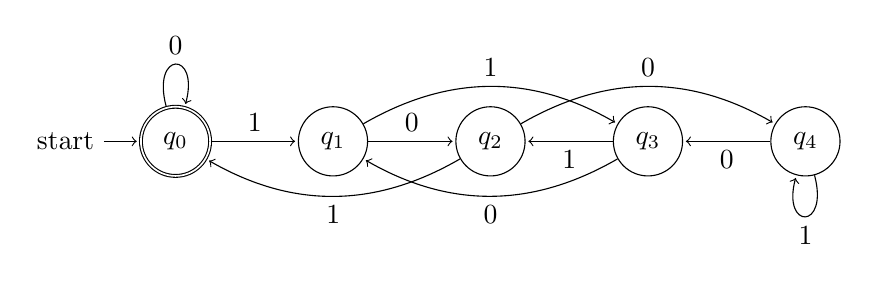
\begin{tikzpicture}[shorten >=1pt,node distance=2cm,on grid,auto]
            \node[state, accepting, initial] (q_0)   {$q_0$};
            \node[state] (q_1) [right=of q_0] {$q_1$};
            \node[state] (q_2) [right=of q_1] {$q_2$};
            \node[state] (q_3) [right=of q_2] {$q_3$};
            \node[state] (q_4) [right=of q_3] {$q_4$};
            \path[->]
                (q_0)
                    edge [loop above] node {0} (q_0)
                    edge node {1} (q_1)
                (q_1)
                    edge node {0} (q_2)
                    edge [bend right=-30] node {1} (q_3)
                (q_2)
                    edge [bend left] node {1} (q_0)
                    edge [bend right=-30] node {0} (q_4)
                (q_3)
                    edge node {1} (q_2)
                    edge [bend left] node {0} (q_1)
                (q_4)
                    edge node {0} (q_3)
                    edge [loop below] node {1} (q_4);
        \end{tikzpicture}
        \caption{DFA, \(A\), this is really beautiful, ya know?}
        \label{fig:multiple5}
    \end{figure}

    \textbf{Justification}
    \\

    Take a given binary number, \(x\). Since there are only two inputs to our
    state machine, \(x\) can either become \(x0\) or \(x1\). When a 0 comes
    into the state machine, it is the same as taking the binary number and
    multiplying it by two. When a 1 comes into the machine, it is the same as
    multipying by two and adding one.
    \\

    Using this knowledge, we can construct a transition table that tell us
    where to go:

    \begin{table}[ht]
        \centering
        \begin{tabular}{c || c | c | c | c | c}
            & \(x \mod 5 = 0\)
            & \(x \mod 5 = 1\)
            & \(x \mod 5 = 2\)
            & \(x \mod 5 = 3\)
            & \(x \mod 5 = 4\)
            \\
            \hline
            \(x0\) & 0 & 2 & 4 & 1 & 3 \\
            \(x1\) & 1 & 3 & 0 & 2 & 4 \\
        \end{tabular}
    \end{table}

    Therefore on state \(q_0\) or (\(x \mod 5 = 0\)), a transition line should
    go to state \(q_0\) for the input 0 and a line should go to state \(q_1\)
    for input 1. Continuing this gives us the Figure~\ref{fig:multiple5}.
\end{homeworkProblem}

\begin{homeworkProblem}
    Write part of \alg{Quick-Sort($list, start, end$)}

    \begin{algorithm}[]
        \begin{algorithmic}[1]
            \Function{Quick-Sort}{$list, start, end$}
                \If{$start \geq end$}
                    \State{} \Return{}
                \EndIf{}
                \State{} $mid \gets \Call{Partition}{list, start, end}$
                \State{} \Call{Quick-Sort}{$list, start, mid - 1$}
                \State{} \Call{Quick-Sort}{$list, mid + 1, end$}
            \EndFunction{}
        \end{algorithmic}
        \caption{Start of QuickSort}
    \end{algorithm}
\end{homeworkProblem}

\pagebreak

\begin{homeworkProblem}
    Suppose we would like to fit a straight line through the origin, i.e.,
    \(Y_i = \beta_1 x_i + e_i\) with \(i = 1, \ldots, n\), \(\E [e_i] = 0\),
    and \(\Var [e_i] = \sigma^2_e\) and \(\Cov[e_i, e_j] = 0, \forall i \neq
    j\).
    \\

    \part

    Find the least squares esimator for \(\hat{\beta_1}\) for the slope
    \(\beta_1\).
    \\

    \solution

    To find the least squares estimator, we should minimize our Residual Sum
    of Squares, RSS:

    \[
        \begin{split}
            RSS &= \sum_{i = 1}^{n} {(Y_i - \hat{Y_i})}^2
            \\
            &= \sum_{i = 1}^{n} {(Y_i - \hat{\beta_1} x_i)}^2
        \end{split}
    \]

    By taking the partial derivative in respect to \(\hat{\beta_1}\), we get:

    \[
        \pderiv{
            \hat{\beta_1}
        }{RSS}
        = -2 \sum_{i = 1}^{n} {x_i (Y_i - \hat{\beta_1} x_i)}
        = 0
    \]

    This gives us:

    \[
        \begin{split}
            \sum_{i = 1}^{n} {x_i (Y_i - \hat{\beta_1} x_i)}
            &= \sum_{i = 1}^{n} {x_i Y_i} - \sum_{i = 1}^{n} \hat{\beta_1} x_i^2
            \\
            &= \sum_{i = 1}^{n} {x_i Y_i} - \hat{\beta_1}\sum_{i = 1}^{n} x_i^2
        \end{split}
    \]

    Solving for \(\hat{\beta_1}\) gives the final estimator for \(\beta_1\):

    \[
        \begin{split}
            \hat{\beta_1}
            &= \frac{
                \sum {x_i Y_i}
            }{
                \sum x_i^2
            }
        \end{split}
    \]

    \pagebreak

    \part

    Calculate the bias and the variance for the estimated slope
    \(\hat{\beta_1}\).
    \\

    \solution

    For the bias, we need to calculate the expected value
    \(\E[\hat{\beta_1}]\):

    \[
        \begin{split}
            \E[\hat{\beta_1}]
            &= \E \left[ \frac{
                \sum {x_i Y_i}
            }{
                \sum x_i^2
            }\right]
            \\
            &= \frac{
                \sum {x_i \E[Y_i]}
            }{
                \sum x_i^2
            }
            \\
            &= \frac{
                \sum {x_i (\beta_1 x_i)}
            }{
                \sum x_i^2
            }
            \\
            &= \frac{
                \sum {x_i^2 \beta_1}
            }{
                \sum x_i^2
            }
            \\
            &= \beta_1 \frac{
                \sum {x_i^2 \beta_1}
            }{
                \sum x_i^2
            }
            \\
            &= \beta_1
        \end{split}
    \]

    Thus since our estimator's expected value is \(\beta_1\), we can conclude
    that the bias of our estimator is 0.
    \\

    For the variance:

    \[
        \begin{split}
            \Var[\hat{\beta_1}]
            &= \Var \left[ \frac{
                \sum {x_i Y_i}
            }{
                \sum x_i^2
            }\right]
            \\
            &=
            \frac{
                \sum {x_i^2}
            }{
                \sum x_i^2 \sum x_i^2
            } \Var[Y_i]
            \\
            &=
            \frac{
                \sum {x_i^2}
            }{
                \sum x_i^2 \sum x_i^2
            } \Var[Y_i]
            \\
            &=
            \frac{
                1
            }{
                \sum x_i^2
            } \Var[Y_i]
            \\
            &=
            \frac{
                1
            }{
                \sum x_i^2
            } \sigma^2
            \\
            &=
            \frac{
                \sigma^2
            }{
                \sum x_i^2
            }
        \end{split}
    \]

\end{homeworkProblem}

\pagebreak

\begin{homeworkProblem}
    Prove a polynomial of degree \(k\), \(a_kn^k + a_{k - 1}n^{k - 1} + \hdots
    + a_1n^1 + a_0n^0\) is a member of \(\Theta(n^k)\) where \(a_k \hdots a_0\)
    are nonnegative constants.

    \begin{proof}
        To prove that \(a_kn^k + a_{k - 1}n^{k - 1} + \hdots + a_1n^1 +
        a_0n^0\), we must show the following:

        \[
            \exists c_1 \exists c_2 \forall n \geq n_0,\ {c_1 \cdot g(n) \leq
            f(n) \leq c_2 \cdot g(n)}
        \]

        For the first inequality, it is easy to see that it holds because no
        matter what the constants are, \(n^k \leq a_kn^k + a_{k - 1}n^{k - 1} +
        \hdots + a_1n^1 + a_0n^0\) even if \(c_1 = 1\) and \(n_0 = 1\).  This
        is because \(n^k \leq c_1 \cdot a_kn^k\) for any nonnegative constant,
        \(c_1\) and \(a_k\).
        \\

        Taking the second inequality, we prove it in the following way.
        By summation, \(\sum\limits_{i=0}^k a_i\) will give us a new constant,
        \(A\). By taking this value of \(A\), we can then do the following:

        \[
            \begin{split}
                a_kn^k + a_{k - 1}n^{k - 1} + \hdots + a_1n^1 + a_0n^0 &=
                \\
                &\leq (a_k + a_{k - 1} \hdots a_1 + a_0) \cdot n^k
                \\
                &= A \cdot n^k
                \\
                &\leq c_2 \cdot n^k
            \end{split}
        \]

        where \(n_0 = 1\) and \(c_2 = A\). \(c_2\) is just a constant. Thus the
        proof is complete.
    \end{proof}
\end{homeworkProblem}

\end{document}
